\documentclass[prb,preprint]{revtex4-1} 

\usepackage{amsmath}  
\usepackage{amsfonts} 
\usepackage{graphicx} 
\usepackage{color}
\usepackage{ulem}

\begin{document}


\title{}


\author{Danika Luntz-Martin}
\email{dluntzma@smith.edu}
\affiliation{Department of Physics, Smith College, Northampton, MA 01063}

\author{William Williams}
\email{wwilliams@smith.edu} 
\affiliation{Department of Physics, Smith College, Northampton, MA 01063}

\date{\today}

\begin{abstract}


\end{abstract}


\maketitle 


\section{Introduction} 


\section{Theory}

Krypton is one of the noble gases; its outer electron shell is completely filled therefore the energy gap between the ground energy state and the first excited state is large. Therefore to laser cool from the ground state would require 123.5nm light which is not currently experimentally possible. To be able to trap krypton atoms they need to be in an excited state and that state needs to be metastable so that the atoms cannot decay while we are cooling and trapping them. Krypton has a metastable state that is 760 nm below the first accessible excited state from which it is possible to cool and trap.

To get the kryptons to the metastable state we used a 215nm light to drive a two-photon transition from the ground $4P^6$ $^1S_0$ state, to the $5P_{[3/2]_2}$ state, see Figure~\ref{KrEnergyLevels}. Throughout our calculations we call the ground $4P^6$ $^1S_0$ state 'state 1' and the $5P_{[3/2]_2}$ state 'state 2.' There are other states at similar energies to the states in question, but they are not important for our experiment because transitions to them are quantum mechanically forbidden. From the $5P_{[3/2]_2}$ state the atom will either decay to the ground state or it will decay to a metastable state, the $5S_{[3/2]_2}$ state. We called this metastable state 'state 3.' The last possibility is that the atom can ionize either from the the $5P_{[3/2]_2}$ state or the metastable $5S_{[3/2]_2}$ state. 

\begin{figure}[h!]
\centering
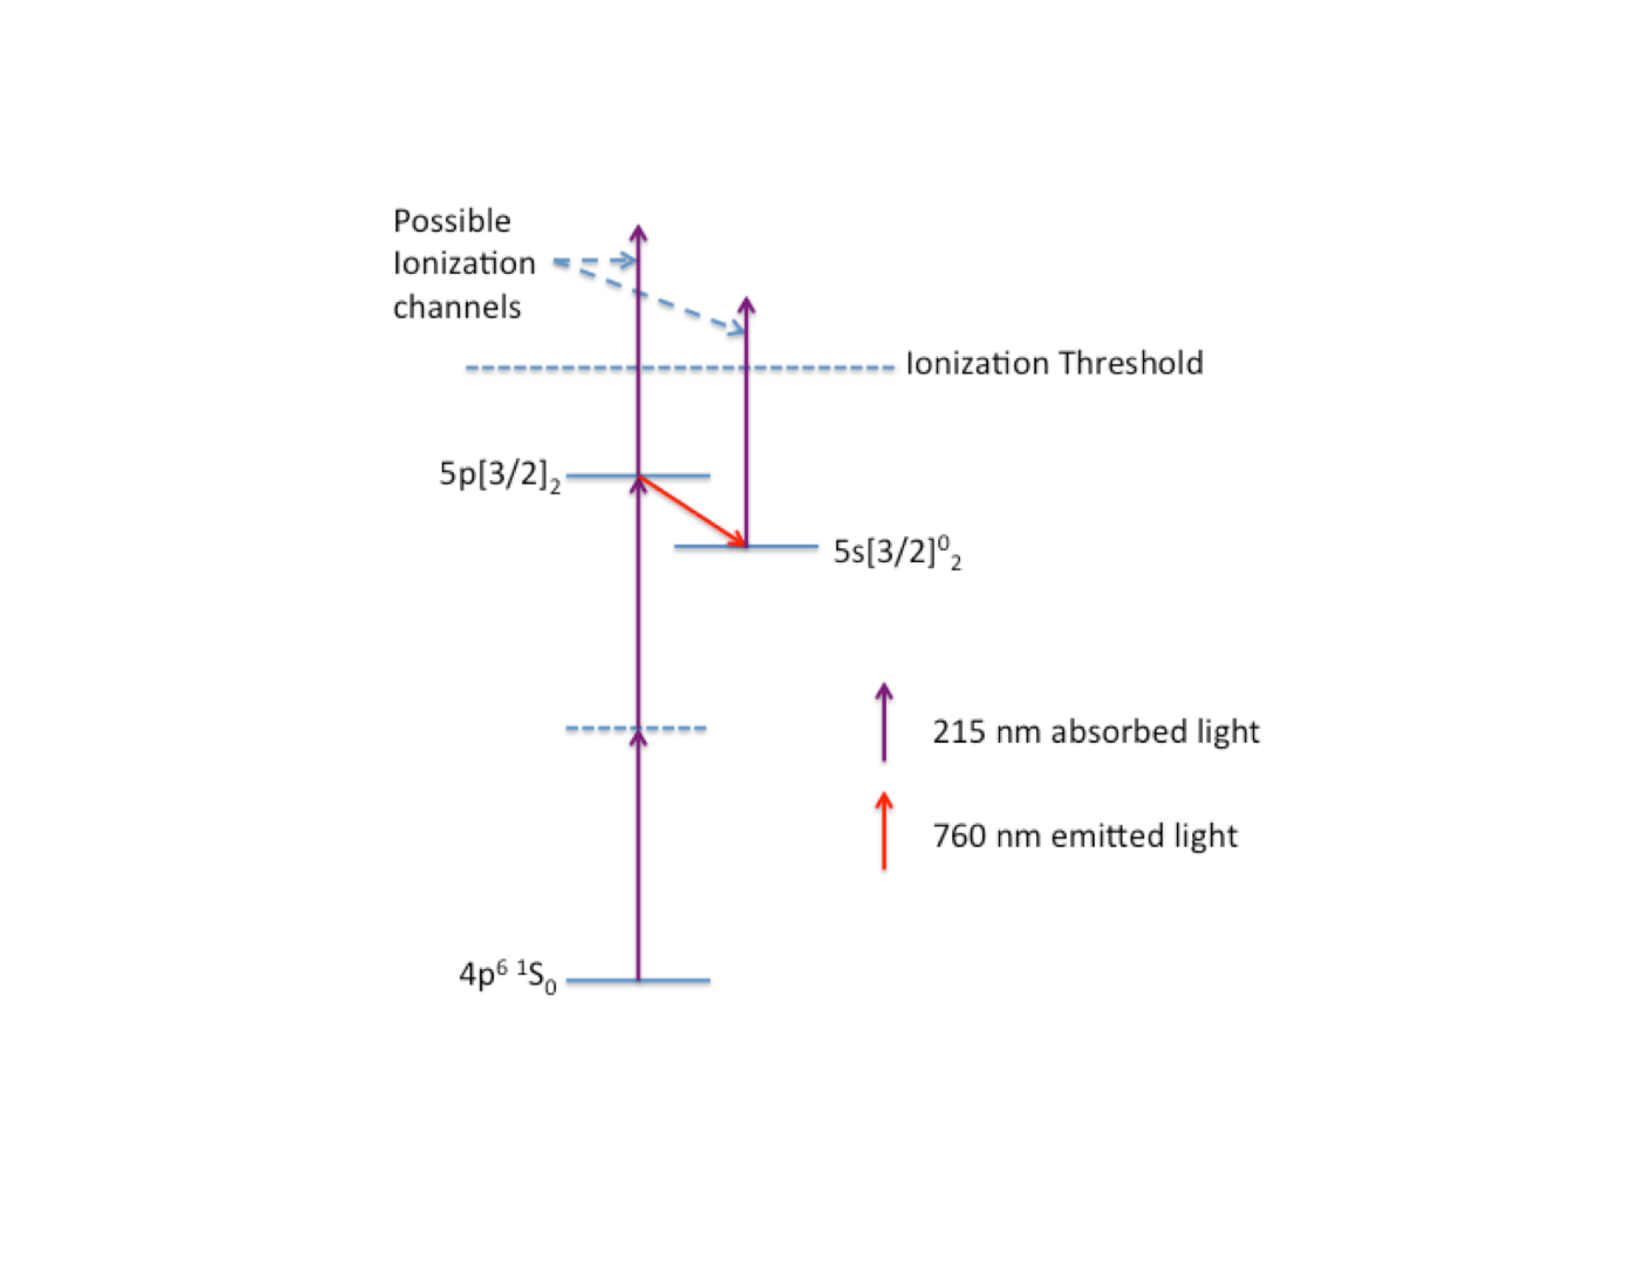
\includegraphics[width=6in]{KrEnergyLevels.pdf}
\caption{The energy levels of krypton. This figure only includes energy levels that are relevant to our experiment. Atoms are excited from the $4P^6$ $^1S_0$ state using two-photons to the $5P_{[3/2]_2}$ state then they decay either back to the $4P^6$ $^1S_0$ state or to the $5S_{[3/2]_2}$ state. Atoms can be ionized from both the $5S_{[3/2]_2}$ state and the $5P_{[3/2]_2}$ state.}
\label{KrEnergyLevels}
\end{figure}


Atom trap trace analysis counts atoms that have been trapped so it is limited by the number of atoms in the metastable state, i.e. the number of atoms available to be trapped. To determine the efficiency of our set up, we calculated the percentage of krypton atoms that ended up in the metastable $5S_{[3/2]_2}$ state using the rate equations.

\begin{equation}
\label{RateEq1}
\frac{dN_1}{dt} = -\omega_{12}N_1 + \frac{1}{\tau_{21}}N_2
\end{equation}

Equation~\ref{RateEq1} gives the rate of change in the number of atoms ($N_1$) in the ground state. $\omega_{12}$ is the rate by which atoms in state 1 (the ground state) which are excited to state 2, the $5P_{[3/2]_2}$ state, via the two-photon transition. $\omega_{12}$ is negative because atoms are leaving state 1. $\frac{1}{\tau_{21}}$ is the rate of decay from state 2 back to state 1. Similarly, there are differential equations for the three other states.

\begin{equation}
\label{RateEq2}
\frac{dN_2}{dt} = \omega_{12}N_1 -  \frac{1}{\tau_{21}}N_2 - \frac{1}{\tau_{23}}N_2 - R_2N_2
\end{equation}

\begin{equation}
\label{RateEq3}
\frac{dN_3}{dt} =  \frac{1}{\tau_{23}}N_2 - R_3N_3
\end{equation}

\begin{equation}
\label{RateEq4}
\frac{dN_4}{dt} = R_2N_2 + R_3N_3
\end{equation}

Where $\tau_{23}$ is the decay rate from state 3, the metastable state, to state 2. $R_2$ and $R_3$ are the ionization rates from states 2 and 3 respectively. $N_4$ is the number of atoms which have been ionized, just as $N_2$ and $N_3$ are the number of atoms in state 2 and state 3.

Solving these linearly dependent equations is possible, but the computational time is much shorter if they are put into matrix form.

\begin{equation}
\label{RateEqMatrix}
\begin{bmatrix}
	\frac{dN_1}{dt} \\
	\frac{dN_2}{dt} \\
	\frac{dN_3}{dt} \\
	\frac{dN_4}{dt} \\
\end{bmatrix}
=
\begin{pmatrix}
	-\omega_{12} & \frac{1}{\tau_{21}}  & 0 &  0   \\
	\omega_{12}  & -\frac{1}{\tau_{21}}- \frac{1}{\tau_{23}}-R_2 & 0 & 0 \\
	0  &  \frac{1}{\tau_{23}}  & - R_3 & 0 \\
	0  &  R_2  & R_3 & 0  \\
\end{pmatrix}
\begin{bmatrix}
	N_1 \\
	N_2 \\
	N_3 \\
	N_4 \\
\end{bmatrix}
\end{equation}

The general solution to the first order differential matrix equation is

\begin{equation}
\label{RateEqSol}
N(t) = A_1e^{\lambda_1 t} v_1 + A_2e^{\lambda_2 t} v_2 + A_3e^{\lambda_3 t} v_3 + A_4e^{\lambda_4 t} v_4 
\end{equation}

where $\lambda$ is an eigenvalue of the matrix and $v$ is an eigenvector of the matrix.  A is the amplitude determined by the initial conditions. The initial condition is that all of the atoms are in the ground state, state 1. That is

\begin{equation}
\label{InitialCond}
N_1(0) = 1, \	\	\	\	
N_2(0) = 0, \	\	\	\	
N_3(0) = 0, \	\	\	\	
N_4(0) = 0 
\end{equation}

which allows us to obtain particular solutions to the rate equations. We did all calculations and analysis in Mathematica. Once we had the solutions to the rate equations we needed to define the variables $\omega_{12}$, $\tau_{21}$, $\tau_{23}$, $R_2$ and $R_3$ which make up the eigenvectors and eigenvalues of the matrix.

\subsection{Constant Intensity and Velocity Approximation} 

For our initial calculation we made a couple simplifying approximations. The first approximation we made was to model the beam profile as constant. The second approximation was to use a single averaged velocity rather then the Maxwell velocity distribution. We later expanded our calculations to account for the beam profile and the velocity distribution those calculations can be found in the subsequent sections. 

The decay rates for state 2 ($5P_{[3/2]_2}$) to state 1 (ground state) and state 3 (metastable state) are know quantities.
\begin{equation}
\label{DecayRates} 
\tau_{21} = 1.1x10^7 s, \	\	\	\	 \tau_{23} = 3.1x10^7s
\end{equation} 
\textcolor{blue}{Does NIST have these? I didn't see them cited in the MRI proposal.}

The ionization rates are given by 
\begin{equation}
\label{IonizationRates}
R = \sigma_{pi} \frac{I}{\hbar\omega}
\end{equation}

where $I$ is the intensity of the laser calculated from power, $I = \frac{P}{\frac{1}{2}\pi w^2}$ and $w$ is the beam waist. We used a power value of $7.5 W$ based on a conservative estimate from the laser specifications. $\omega$ is the frequency of the light defined as $\omega = \frac{2\pi c}{\lambda}$. $\sigma_{pi}$ is the photo-ionization cross section, the probability that a photon will be absorbed by the atom. $\sigma_{pi2} = .5$ Mbarn for the $5P_{[3/2]_2}$ state and $\sigma_{pi2} = .25$ Mbarn for the $5S_{[3/2]_2}$ state.~\cite{Cannon}

The rate by which atoms are excited by two-photon transition from state 1 to state 2 is $\omega_{12}$ given by

\begin{equation}
\label{ExcitationRate}
\omega_{12} = \sigma_0 g \frac{I^2}{(\hbar \omega)^2}
\end{equation}

$\sigma_0$ is the two-photon cross section, the probability that two photons will be absorbed, which is $4.4x10^{-35} cm^{-4}$.~\cite{NIST} $g$ is the on resonance line shape factor, defined as 

\begin{equation}
\label{LineShapeFactor}
g = 2 \sqrt{\frac{Log(2)}{2 \pi (\Delta \omega_L^2 + \Delta \omega_D^2)}}
\end{equation}

with $\Delta\omega_L$ as the line width of the laser. $\Delta \omega_D$ is Doppler line width for the two-photon transition, which is zero in our case because the krypton atoms are moving perpendicular to the laser.

The solution to these equations is given in Figure~\ref{MetaGraph1} which shows the fraction of atoms in the metastable state as a function of the size of the laser's beam waist. The optimum number of atoms end up in the metastable state when the beam waist is close to 20 microns. When the beam waist is smaller than 20 microns most of the atoms do not have time to reach the excited state as they pass through the laser beam. When the beam waist is larger than 20 microns, atoms from the metastable state are ionized.

\begin{figure}[h!]
\centering
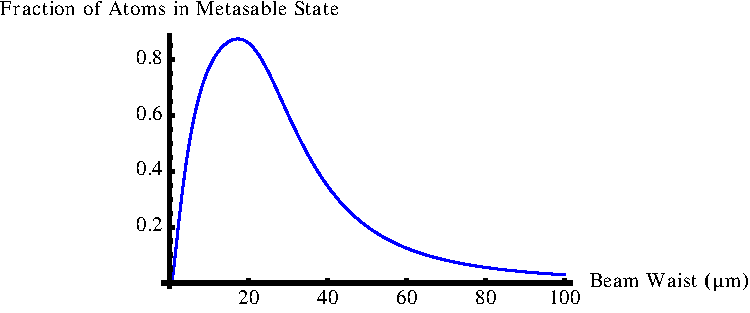
\includegraphics[width=6in]{MetaGraph1.pdf}
\caption{The fraction of atoms in the metastable state as a function of laser's beam waist. The fraction of atoms reaching the metastable state increases sharply as the beam waist increases until 20 microns. After 20 microns the number of atoms in the metastable state decreases because the atoms are ionizing.}
\label{MetaGraph1}
\end{figure}

Figure~\ref{TimeGraph} shows the fraction of atoms in each of the states which is helpful to see how the atoms move between states. The green line is the ground state which starts at one because the initial condition is all of the atoms in the ground state and continuously decreases as time passes. State 1 is the orange line; it quickly increases as atoms are excited through two-photon transition. The number of atoms in state 1 decrease as atoms decay either back to the ground state or to the metastable state. The number of atoms in the metastable state increases as atoms decay to it from the state 1. Atoms only leave the metastable state if they ionize. Only a small fraction of atoms are ionized, see the red line.

\begin{figure}[h!]
\centering
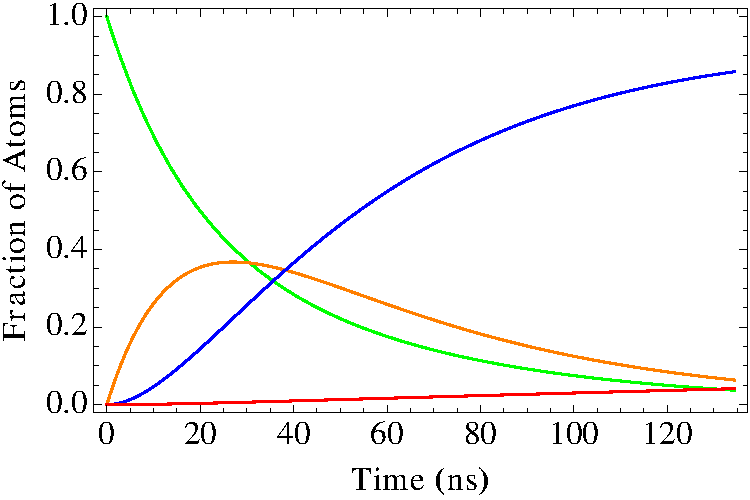
\includegraphics[width=6in]{TimeGraph.pdf}
\caption{The fraction of atoms in each state plotted against time. The green line is the ground state. The orange line is the excited $5P_{[3/2]_2}$ state. Blue is the metastable $5S_{[3/2]_2}$ and red is the fraction of atoms that have ionized.}
\label{TimeGraph}
\end{figure}

\subsection{Gaussian Beam Profile}

To make our model more accurate we factored in the intensity profile of the laser beam. From the laser manufacturer's, M Squared, specifications we know that the Ti:Sapphire laser's intensity profile is a two-dimensional gaussian. It was conceptually simple to incorporate the intensity profile into our previous calculation in place of the constant intensity. Computationally, it was not quite as easy.

We replaced our former intensity with by $I = I_0 e^{\frac{-2 x^2}{w^2}}$ where $I_0 = \frac{P}{\frac{1}{2}\pi w^2}$, the same intensity we used as a constant in our previous approximation. However, the addition of the gaussian term means that the equations no longer have analytical solutions. We solved the differential equations numerically.

The resulting graph is noticeably different from our first approximation, see Figure~\ref{AllGraph}. Adding the intensity profile does not change the shape of the peak, but it does make the peak lower and narrower. The location of the peak is now around 15 micrometers, rather than the 20 micrometers from the constant intensity approximation.  The fraction of atoms reaching the metastable state is still quite high having been decreased by just over five percent from roughly .9 to .85.

\begin{figure}[h!]
\centering
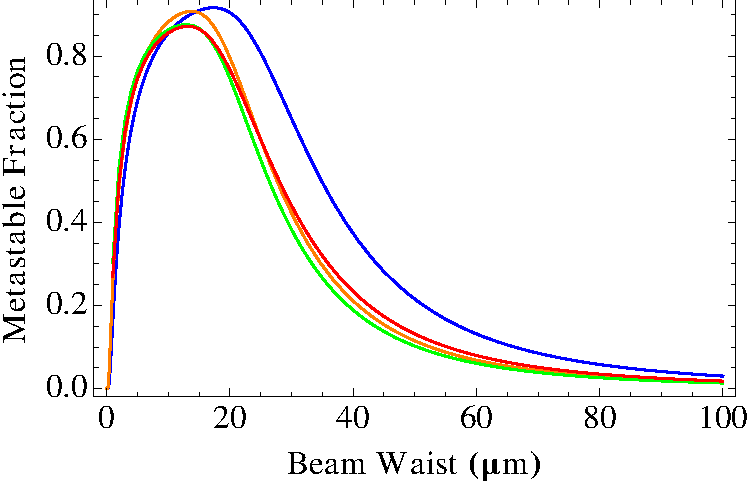
\includegraphics[width=6in]{AllGraph.pdf}
\caption{The blue line represents the calculation assuming root-mean-square velocity and a constant intensity. The green line represents the calculation assuming the root-mean-square velocity and a gaussian intensity profile. Finally, the red line is the calculation using both the gaussian intensity profile and the Maxwell velocity distribution. The root-mean-square velocity is a good approximation the green and red lines are very close. The constant intensity is not as good an approximation for the more accurate gaussian intensity profile, note the differences between blue line and the green line.}
\label{AllGraph}
\end{figure}


\subsection{Maxwell Velocity Distribution}

Adding the Maxwell velocity distribution presents new difficulties. To account for the range of velocities we first calculated the fraction of atoms in each of a series of intervals. Then we calculated the fraction of atoms from each interval, that is at each different velocity, that reach the metastable state. We then multiplied the fraction of atoms that reach the metastable state from a velocity interval by the fraction of atoms in that velocity interval. Then we added together the resulting fraction from each interval to obtain the total fraction of atoms that end up in the metastable state. See Figure~\ref{AllGraph} for a comparison of the fraction of atoms reaching the metastable state from each calculation.

Modeling the velocity of the atoms as the root-mean-square velocity is a very good approximation. The differences between using the root-mean-square velocity as a single average value and using the Maxwell velocity distribution were quite small. See the similarity between the green and red lines in Figure~\ref{AllGraph}.

The fraction of atoms reaching the metastable state is constant through time. The number of atoms that are in the metastable state at a specific time does change, look back to Figure~\ref{TimeGraph}. The number of atoms in the metastable state increases through time before plateauing. However the total fraction of atoms reaching the metastable is the fraction of atoms that are currently there plus the fraction of atoms in the excited, second state that will decay into the metastable state. The sum of these two numbers remains constant through time which is why our total calculation is stable through time.

 

\section{Titanium-Sapphire Laser}

A titanium-sapphire (Ti-Sapphire) laser uses titanium doped sapphire crystals, hence the name. These crystals are pumped using another laser. We used a \textcolor{blue}{add specific wavelength and type.} Refer to Figure~\ref{LaserSetup} for the experimental set-up of the laser. The pump laser could be operated at various powers which adjusted the overall output of the Ti-Sapphire laser. We operated the pump laser at both 18 W and 12 W.

The first step to operating the laser was to turn on the coolers which cooled the sapphire crystals and the pump laser and then to turn on the pump laser and allow it to warm up and stabilize. The pump laser takes around thirty minutes to warm up, before it is warm it will not generate any light from the Ti-Sapphire laser. It is preferable to allow the pump laser longer to fully stabilize because any drift in the pump laser will cause the Ti-Sapphire deviate from optimum and likely lose lock.

Once the pump laser is warm and stable the light into the Ti-Sapphire laser must be optimized. The the output from the pump laser passes first through a beam splitter, then through a set of mirrors which can be used to align the beam in all three axis directions. The power to the Ti-Sapphire laser can be measured by using the beam splitter after the Ti-Sapphire laser and reference cavity, again see Figure~\ref{LaserSetup}. 



\section{Laser Stabilization}

\section{Appendix}

\textcolor{magenta}{Put Mathematica notebooks here!}


\begin{thebibliography}{2}

\bibitem{NIST} A. Kramida, Yu. Ralchenko, J. Reader, J. and NIST ASD Team (2013). NIST Atomic Spectra Database (version 5.1), [Online]. Available: \url{<http://physics.nist.gov/asd>} [Wednesday, 15-Jan-201422:06:55 EST]. National Institute of Standards and Technology, Gaithersburg, MD.

\bibitem{Cannon} B. D. Cannon, ``Model calculations of continuous-wave laser ionization of krypton,'' PNNL-12253 (1999)

\end{thebibliography}


\end{document}
